\documentclass{beamer}
\mode<presentation>{
	\usetheme{Madrid}
}

\usepackage{graphicx}
\usepackage{algorithm}
\usepackage{algpseudocode}
\usepackage{booktabs}

\usepackage{tikz}
\usepackage{amsmath}
\usetikzlibrary{matrix}

\title[University of Connecticut] {Hidden Markov Models in Biological Sequence Analysis}

\author{Huyen D. Nguyen}

\institute[]{University of Connecticut \\
	\medskip
	\text{Department of Statistics}\\
}
\date{November 06, 2023}

\begin{document}
\begin{frame}
	\titlepage
\end{frame}

\begin{frame}{Introduction: Hidden Markov Model}
	\begin{itemize}
		\item A \textbf{hidden Markov Model (HMM)} is a statistical model that can be used to describe the evolution of observable events that depend on a Markov process with unobservable states. 
		\item Many real world problems deal with classifying raw observations into a number of categories or class labels that are more meaningful.
		\item HMM applications in signal processing, pattern recognition, economics, finance, bioinformatics, etc.
	\end{itemize}
\end{frame}

\begin{frame}{Introduction: Biological Sequence Analysis}
	\begin{itemize}
		\item The modeling approach of HMM is useful in modeling biological sequencess.
		\item Example: Proteins generally consists of multiple domains \cite{yoon2009hidden}. 
		\begin{enumerate}
			\item Predict the constituting domains (one or more hidden Markov states) and their location in amino acid sequences (observations).
			\item Find the protein family that the a protein sequence belongs.
		\end{enumerate}
	\end{itemize}
\end{frame}

\begin{frame}{Outline}
	\tableofcontents
\end{frame}

\section{Overview of Hidden Markov Model}
\begin{frame}{HMM Definition}
	\begin{itemize}
		\item A set of $N$  hidden states, $ Q = q_1 q_2\cdots q_N.$
		\item A transition probability matrix $A$, each $a_{ij}$ representing the probability of moving state $i$ to state $j$, s.t $\sum_{j=1}^{N} a_{ij} = 1 \forall i$.
		\item A sequence of $T$ observations, $ O = o_1 o_2\cdots o_T$, each one drawn from a set $V = v_1, v_2, \cdots, v_V$.
		\item A sequence of emission probabilities, $B = b_i(o_t)$,  each expressing the probability of an observation $o_t$ being generated from state $i$.
		\item An initial probability distribution over states, $\pi = \pi_1, \pi_2,\cdots, \pi_N$. $\pi_i$ is the probability that the Markov chain will start in state $i$. $\sum_{i=1}^{N} \pi_i = 1$.
	\end{itemize}
\end{frame}

\begin{frame}{HMM Definition}
	\begin{itemize}
		\item Markov Assumption: the probability of a particular state depends only on the previous state
		\begin{equation}
			\begin{split}
				P(q_i \vert q_1\cdots q_{i-1}) = P(q_i \vert q_{i-1}).
			\end{split}
		\end{equation}
		\item Output Independence: the probability of an output observation $o_i$ depends only on the state that produced the observation $q_i$ and not on previous states or observations
		\begin{equation}
			\begin{split}
				P(o_i \vert q_1,\cdots q_T, o_1,\cdots , o_T) = P(o_i \vert q_i) .
			\end{split}
		\end{equation}
	\end{itemize}
	\begin{figure}
		\centering
		\resizebox{3in}{!}{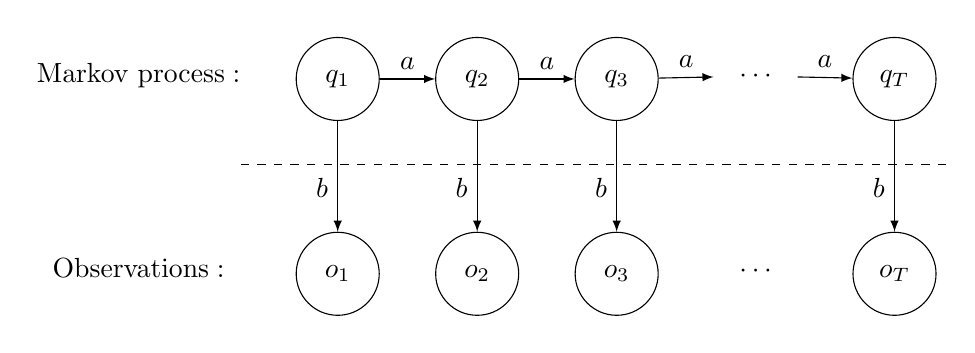
\begin{tikzpicture}
				\matrix[matrix of math nodes,column sep=2em,row
				sep=4em,cells={nodes={circle,draw,minimum width=3em,inner sep=0pt}},
				column 1/.style={nodes={rectangle,draw=none}},
				column 5/.style={nodes={rectangle,draw=none}},
				ampersand replacement=\&] (m) {
					\text{Markov process}: \&
					q_1 \& q_2 \& q_3 \& \cdots \& q_{T}\\
					\text{Observations}: \& 
					o_1 \& o_2 \& o_3 \& \cdots \& o_{T}\\
				};
				\foreach \X in {2,3,4,5}
				{\draw[-latex] (m-1-\X) -- (m-1-\the\numexpr\X+1) node[midway,above]{$a$};
					\ifnum\X=5
					\draw[-latex] (m-1-6) -- (m-2-6) node[pos=0.6,left]{$b$};
					\else
					\draw[-latex] (m-1-\X) -- (m-2-\X) node[pos=0.6,left]{$b$};
					\fi}
				\draw[dashed] ([yshift=1ex]m.east) -- ([yshift=1ex]m.east-|m-1-1.east);
		\end{tikzpicture}}
		\caption{An example of a hidden Markov model.}
		\label{fig:HiddenMarkov}
	\end{figure}
\end{frame}
\section{The Scoring Problem and the Forward Algorithm}
\begin{frame}{The Scoring Problem and the Forward Algorithm}
	\begin{block}{The Scoring Problem}
		Given a HMM $\lambda = (A,B)$ and a sequence of observation $O$, what is the probability of observing the sequence $P(O \vert \lambda)$?
	\end{block}
	\begin{itemize}
		\item We can compute the probability of the observations by summing over all possible hidden state sequences:
		$$P(O) = \sum_Q P(O, Q) = \sum_Q P(O\vert Q) P(Q).$$
		\item For an HMM with $N$ hidden states and an observation sequence of $T$ observations, there are $N^T$ possible hidden sequences.
		\item $N^T$ can get very large.
	\end{itemize}
\end{frame}

\begin{frame}{The Forward Algorithm}
	\begin{itemize}
		\item The forward algorithm is a dynamic programming algorithm. 
		\item The probability of being in state $j$ knowing the first $t$ observaitons, given the model $\lambda$
		\begin{equation}
			\alpha_t(j) = P(o_1\cdots o_t, q_t = j \vert \lambda).
		\end{equation}
		\item $\alpha_t(j)$ is computed recursively by summing over the extensions of all the paths that lead to the current cell
		\begin{equation}
			\alpha_t(j) = \sum_{i=1}^N \alpha_{t-1}(i) a_{ij} b_j (o_t).
		\end{equation}
		\item The probability of observing the sequence
		\begin{equation}
			P(O \vert \lambda) = \sum_{i=1}^N \alpha_T(i).
		\end{equation}
	\end{itemize}
\end{frame}

%\begin{frame}{The Forward Algorithm}
%	\begin{enumerate}
%		\item Initialization:
%		$$ \alpha_t(j) = \pi_j b_j(o_1), \quad 1 \leq j \leq N.$$
%		\item Recursion:
%		$$\alpha_t(j) = \sum_{i=1}^N \alpha_{t-1}(i) a_{ij} b_j (o_t), \quad 1 \leq j \leq N, 1 < t <T.$$
%		\item Termination:
%		$$P(O \vert \lambda) = \sum_{i=1}^N \alpha_T(i).$$
%	\end{enumerate}
%\end{frame}


\section{The Decoding Problem and the Viberti Algorithm}
\begin{frame}{The Decoding Problem }
	\begin{block}{The Decoding Problem}
		Given a HMM $\lambda = (A,B)$ and a sequence of observation $O$, find the most probable hidden state sequence $Q$.
	\end{block}
	\begin{itemize}
		\item Run the forward algorithm and compute the likelihood of the observation sequence given each hidden state sequence.
		\item Choose the hidden state sequence with the maximum observation likelihood.
		\item We can get too many hidden state sequences.
	\end{itemize}
\end{frame}

\begin{frame}{Viberti Algorithm}
	\begin{itemize}
		\item Viberti algorithm is also a dynamic programming algorithm.
		\item The probability of the most probable state sequence $q_1, \cdots, q_{t-1}$ given the model $\lambda$
		\begin{equation}
			v_t(j) = \max_{q_1\cdots q_{t-1}} P(q_1\cdots q_{t-1}, o_1\cdots o_{t-1}, q_t = j \vert \lambda).
		\end{equation}
		\item $v_t(j)$ is computed it recursively it 
		\begin{equation}
			v_t(j) = \max_i[v_{t-1}(i) a_{ij} b_j(o_t)].
		\end{equation}
		\item The opimal path can be found by tracing back the recusions that led to the maximum probability.
	\end{itemize}
\end{frame}


\begin{frame}{Decoding Problem: CG island example}
	\begin{itemize}
		\item In genome, the frequency of CG dinucleotide is relative low (about 1\% in human genome) because of methylation. 
		\item The resulting methylated cytosine has the tendency to further deaminate into thymine \cite{compeau2018bioinformatics}.
		\item However, mythelation is often suppressed around genes, particularly near transcriptional start sites.
		\item These areas are called CG islands, where CG appears relatively frequently compared to the rest of the genome.
		\item Identifying CG islands is useful in identifying different genes.
	\end{itemize}
\end{frame}

\begin{frame}{HMM for Decoding Problem}
	\begin{itemize}
		\item CG Island Decoding Problem: Given an RNA sequence, we want to identify the high CG content region and low CG content region.
		\item HMM for Decoding Problem: Given a symbol sequence \textbf{X}, find optimal state sequence or optimal path in the HMM that maximizes the observation probability of the given sequence.
	\end{itemize}
\end{frame}

\begin{frame}{HMM for Decoding Problem}
	Example 1 \cite{borodovsky2006problems}: Consider the sequence S = \textbf{GGCACTGAA} and the initial, transition, and emission probability as in the following graph
	\begin{figure}
		\centering
		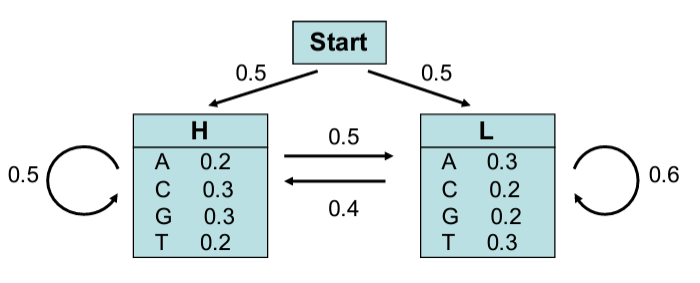
\includegraphics[width = 0.7\textwidth]{example1.png}
		\label{fig:example1}
		\caption{Example of HMM for CG island problem: 2 hidden Markov states H (high CG content) and L (low CG content), 4 observable symbols A,T C,G.}
	\end{figure}
\end{frame} 

\begin{frame}{Viberti Algorithm}
	Back to example 1: The most probable path (sequence of hidden states) is \textbf{HHHLLLLLL} and its probability is $2^{-24.49} = 4.25 \times 10^{-8}$.
	\begin{figure}
		\centering
		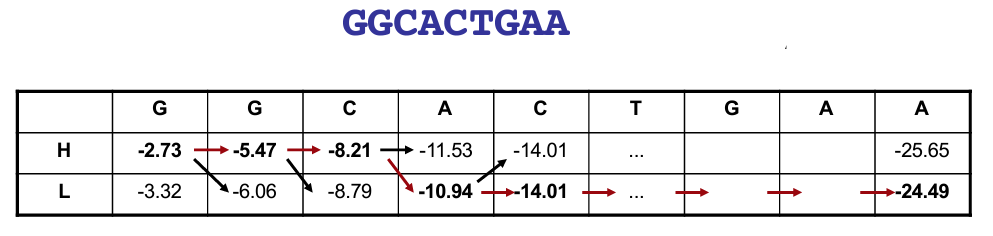
\includegraphics[width = 0.7\textwidth]{example1cal.png}
		\label{fig:example2cal}
		\caption{Viberti algorithm calculation for example 1 using $\log_2$ and back tracing to find the most probable path.}
	\end{figure}
\end{frame}

\section{The Training Problem and the Baum-Welch algorithm}
\begin{frame}{The Training Problem }
	\begin{block}{The Training Problem}
		Given a sequence of observation $O$ and the set of states in the HMM, learn the HMM parameters A and B.
	\end{block}
\end{frame}

\section{Extensions of HMM for Biological Sequence Analysis}
\begin{frame}{References}
	\bibliographystyle{acm}
	\bibliography{refs}
\end{frame}

\end{document}